% Chapitre Méthodologie
\newpage
\chapter{MÉTHODOLOGIE}

Cette section présente en détail l'approche méthodologique développée pour la détection d'intrusions réseau. Notre stratégie repose sur une architecture hiérarchique combinant apprentissage supervisé et non-supervisé, appliquée au jeu de données NSL-KDD. L'ensemble du processus, depuis le prétraitement des données jusqu'à la classification finale, est conçu pour optimiser à la fois la précision de détection et la capacité de discrimination entre les différents types d'attaques.

\section{Architecture générale du système}

Notre système de détection d'intrusions adopte une approche hiérarchique en deux étapes distinctes, illustrée dans la Figure~\ref{fig:pipeline_general}. Cette architecture permet une analyse progressive du trafic réseau, commençant par une classification binaire robuste avant d'affiner la caractérisation des menaces détectées.

\begin{figure}[H]
    \centering
    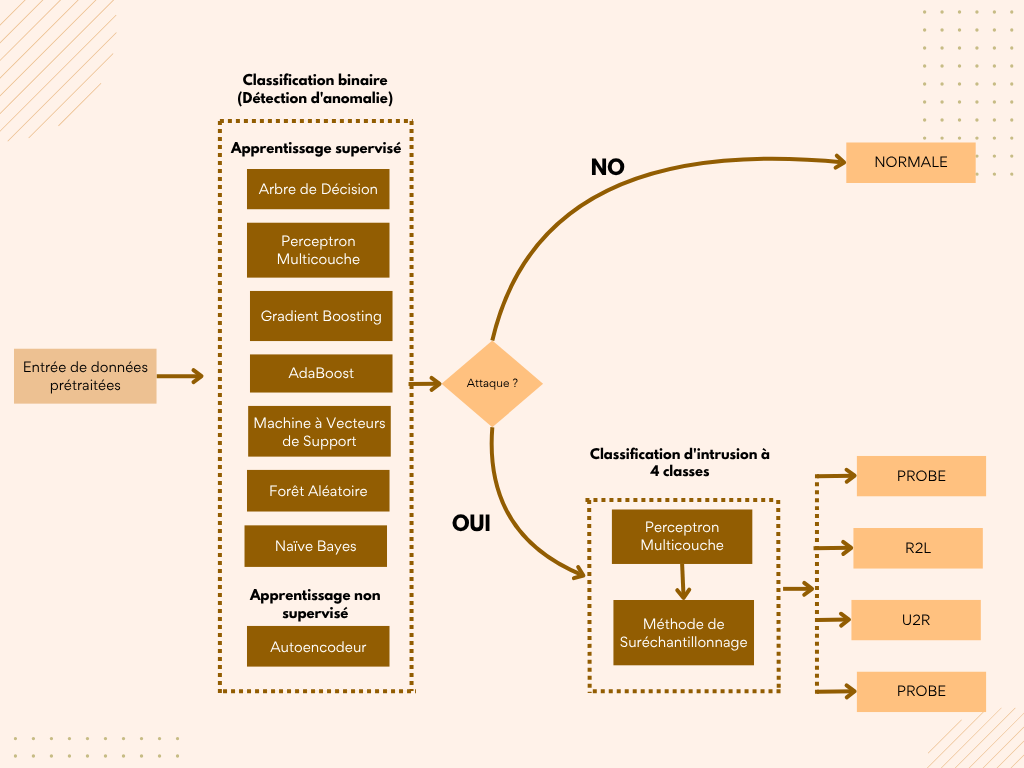
\includegraphics[width=0.8\textwidth]{Assets/ARCHITECTEUR ML.png}
    \caption{Architecture générale du système de détection d'intrusions hiérarchique}
    \label{fig:pipeline_general}
\end{figure}

La première étape effectue une discrimination fondamentale entre le trafic normal et les activités suspectes. Cette phase mobilise plusieurs algorithmes d'apprentissage automatique, incluant des approches supervisées traditionnelles et une méthode non-supervisée basée sur un autoencodeur. La seconde étape se concentre sur la classification fine des intrusions détectées, catégorisant les attaques selon quatre typologies reconnues dans la littérature scientifique.

\section{Jeu de données NSL-KDD}

\subsection{Présentation et structure}

Le jeu de données NSL-KDD constitue une version améliorée du célèbre dataset KDD Cup 99, corrigeant plusieurs limitations de son prédécesseur. Ce dataset comprend 125,973 enregistrements d'entraînement et 22,544 enregistrements de test, chaque instance étant caractérisée par 41 attributs décrivant les propriétés d'une connexion réseau.

\subsection{Description détaillée des 41 caractéristiques}

Les caractéristiques du dataset NSL-KDD se répartissent en trois catégories principales, chacune capturant des aspects différents du comportement réseau :

\subsubsection{Caractéristiques de base (9 attributs)}
Ces attributs sont directement extraits des en-têtes de paquets TCP/IP et représentent les propriétés fondamentales d'une connexion :

\begin{itemize}
    \item \textbf{duration} : Durée de la connexion en secondes
    \item \textbf{protocol\_type} : Type de protocole utilisé (TCP, UDP, ICMP)
    \item \textbf{service} : Service réseau de destination (HTTP, FTP, SMTP, etc.)
    \item \textbf{flag} : État normal ou d'erreur de la connexion (SF, S0, REJ, etc.)
    \item \textbf{src\_bytes} : Nombre d'octets de données transférés de la source vers la destination
    \item \textbf{dst\_bytes} : Nombre d'octets de données transférés de la destination vers la source
    \item \textbf{land} : 1 si la connexion provient et va vers le même hôte/port, 0 sinon
    \item \textbf{wrong\_fragment} : Nombre de fragments incorrects
    \item \textbf{urgent} : Nombre de paquets urgents
\end{itemize}

\subsubsection{Caractéristiques de trafic (13 attributs)}
Ces statistiques sont calculées sur une fenêtre glissante de 100 connexions et analysent les patterns de comportement :

\textbf{Statistiques "même hôte" :}
\begin{itemize}
    \item \textbf{count} : Nombre de connexions vers le même hôte que la connexion courante
    \item \textbf{srv\_count} : Nombre de connexions vers le même service que la connexion courante
    \item \textbf{serror\_rate} : Pourcentage de connexions ayant une erreur SYN
    \item \textbf{srv\_serror\_rate} : Pourcentage de connexions vers le même service ayant une erreur SYN
    \item \textbf{rerror\_rate} : Pourcentage de connexions ayant une erreur REJ
    \item \textbf{srv\_rerror\_rate} : Pourcentage de connexions vers le même service ayant une erreur REJ
    \item \textbf{same\_srv\_rate} : Pourcentage de connexions vers le même service
    \item \textbf{diff\_srv\_rate} : Pourcentage de connexions vers différents services
\end{itemize}

\textbf{Statistiques "hôte de destination" :}
\begin{itemize}
    \item \textbf{dst\_host\_count} : Nombre de connexions ayant le même hôte de destination
    \item \textbf{dst\_host\_srv\_count} : Nombre de connexions ayant le même service de destination
    \item \textbf{dst\_host\_same\_srv\_rate} : Pourcentage de connexions vers le même service de destination
    \item \textbf{dst\_host\_diff\_srv\_rate} : Pourcentage de connexions vers différents services de destination
    \item \textbf{dst\_host\_same\_src\_port\_rate} : Pourcentage de connexions utilisant le même port source
\end{itemize}

\subsubsection{Caractéristiques de contenu (19 attributs)}
Ces attributs analysent le contenu des paquets et sont particulièrement utiles pour détecter les attaques R2L et U2R :

\textbf{Indicateurs d'accès privilégié :}
\begin{itemize}
    \item \textbf{hot} : Nombre d'indicateurs "hot" (accès à fichiers/répertoires sensibles)
    \item \textbf{num\_failed\_logins} : Nombre de tentatives de connexion échouées
    \item \textbf{logged\_in} : 1 si connecté avec succès, 0 sinon
    \item \textbf{num\_compromised} : Nombre de conditions "compromised"
    \item \textbf{root\_shell} : 1 si un shell root a été obtenu, 0 sinon
    \item \textbf{su\_attempted} : 1 si une commande "su root" a été tentée, 0 sinon
\end{itemize}

\textbf{Statistiques d'accès aux fichiers :}
\begin{itemize}
    \item \textbf{num\_root} : Nombre d'accès "root"
    \item \textbf{num\_file\_creations} : Nombre d'opérations de création de fichiers
    \item \textbf{num\_shells} : Nombre d'invitations de commandes shell
    \item \textbf{num\_access\_files} : Nombre d'opérations d'accès aux fichiers de contrôle
    \item \textbf{num\_outbound\_cmds} : Nombre de commandes sortantes dans une session FTP
\end{itemize}

\textbf{Indicateurs de session :}
\begin{itemize}
    \item \textbf{is\_host\_login} : 1 si le login appartient à la liste "hot", 0 sinon
    \item \textbf{is\_guest\_login} : 1 si le login est "guest", 0 sinon
\end{itemize}

\textbf{Statistiques d'erreur de destination :}
\begin{itemize}
    \item \textbf{dst\_host\_srv\_diff\_host\_rate} : Pourcentage de connexions vers différents hôtes
    \item \textbf{dst\_host\_serror\_rate} : Pourcentage de connexions ayant une erreur SYN
    \item \textbf{dst\_host\_srv\_serror\_rate} : Pourcentage de connexions vers le même service ayant une erreur SYN
    \item \textbf{dst\_host\_rerror\_rate} : Pourcentage de connexions ayant une erreur REJ
    \item \textbf{dst\_host\_srv\_rerror\_rate} : Pourcentage de connexions vers le même service ayant une erreur REJ
\end{itemize}

\subsection{Taxonomie des attaques}

NSL-KDD organise les intrusions selon quatre catégories principales, chacune représentant un mode opératoire distinct :

\begin{table}[H]
    \centering
    \caption{Distribution des catégories d'attaques dans NSL-KDD}
    \begin{tabular}{|l|p{6.5cm}|c|}
        \hline
        \textbf{Catégorie} & \textbf{Description} & \textbf{Exemples} \\
        \hline
        DoS & Attaques par déni de service visant à saturer les ressources & neptune, smurf, pod \\
        \hline
        Probe & Tentatives de reconnaissance pour découvrir les vulnérabilités & satan, portsweep, nmap \\
        \hline
        R2L & Intrusions distantes cherchant un accès local non autorisé & warezclient, imap, spy \\
        \hline
        U2R & Élévations de privilèges d'utilisateur vers administrateur & buffer\_overflow, rootkit \\
        \hline
    \end{tabular}
    \label{tab:attack_categories}
\end{table}

\begin{figure}[H]
    \centering
    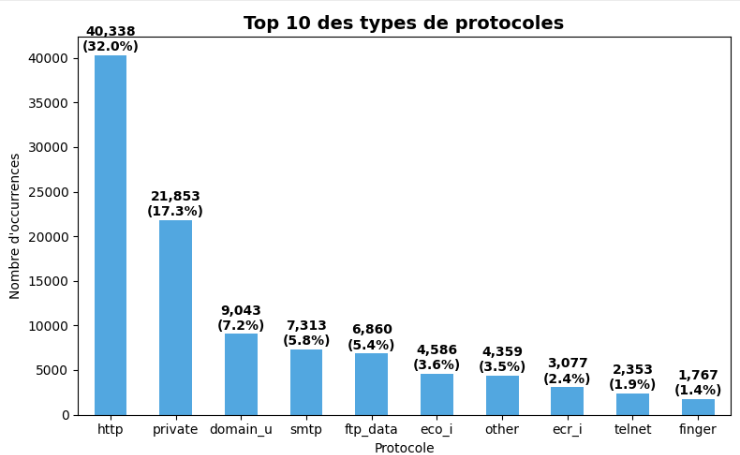
\includegraphics[width=0.8\textwidth]{Assets/Top 10 des types de protocoles.png}
    \caption{Distribution des classes dans le jeu de données NSL-KDD}
    \label{fig:data_distribution}
\end{figure}

\section{Prétraitement des données}

\subsection{Encodage des variables catégorielles}

Le jeu de données NSL-KDD contient trois attributs catégoriels : le type de protocole, le service réseau et l'état de la connexion. Ces variables textuelles nécessitent une transformation numérique pour être exploitables par les algorithmes d'apprentissage automatique.

Nous appliquons un encodage par fréquence (Label Frequency Encoding) qui attribue des valeurs numériques en fonction de la fréquence d'apparition de chaque catégorie. Pour une variable catégorielle $X$ avec des catégories $\{c_1, c_2, ..., c_k\}$, l'encodage par fréquence assigne à chaque catégorie $c_i$ la valeur :

\begin{equation}
    \text{encoded}(c_i) = \text{rank}(\text{freq}(c_i))
\end{equation}

où $\text{freq}(c_i)$ représente la fréquence d'apparition de la catégorie $c_i$ et $\text{rank}$ attribue un rang basé sur cette fréquence.

\subsection{Normalisation des données}

La standardisation des caractéristiques numériques constitue une étape cruciale pour assurer l'efficacité des algorithmes d'apprentissage automatique. Nous appliquons la standardisation Z-score :

\begin{equation}
    z_i = \frac{x_i - \mu}{\sigma}
\end{equation}

où $x_i$ représente la valeur originale, $\mu$ la moyenne arithmétique et $\sigma$ l'écart-type de la caractéristique considérée.

\section{Algorithmes d'apprentissage automatique}

\subsection{Arbres de décision}

Les arbres de décision constituent une famille d'algorithmes d'apprentissage supervisé particulièrement adaptée à l'interprétabilité. Un arbre de décision partitionne récursivement l'espace des caractéristiques en utilisant des tests binaires sur les attributs.

\subsubsection{Critère de division}
Pour construire l'arbre, nous utilisons le critère d'entropie. L'entropie d'un ensemble $S$ est définie par :

\begin{equation}
    H(S) = -\sum_{i=1}^{c} p_i \log_2(p_i)
\end{equation}

où $c$ est le nombre de classes et $p_i$ la proportion d'exemples de classe $i$ dans $S$.

Le gain d'information pour un attribut $A$ divisant $S$ en sous-ensembles \\
$\{S_1, S_2, ..., S_v\}$ est :

\begin{equation}
    \text{Gain}(S,A) = H(S) - \sum_{j=1}^{v} \frac{|S_j|}{|S|} H(S_j)
\end{equation}

\subsubsection{Critère d'arrêt}
L'algorithme s'arrête lorsque :
\begin{itemize}
    \item Tous les exemples appartiennent à la même classe
    \item La profondeur maximale est atteinte
    \item Le nombre minimum d'exemples par feuille est atteint
    \item Le gain d'information est inférieur à un seuil prédéfini
\end{itemize}

\subsection{Forêts aléatoires}

Les forêts aléatoires combinent plusieurs arbres de décision selon le principe du bagging (Bootstrap AGGregatING). Cette méthode d'ensemble améliore la robustesse et la généralisation.

\subsubsection{Algorithme de construction}
Pour construire une forêt de $T$ arbres :

\begin{enumerate}
    \item Pour $t = 1$ à $T$ :
    \begin{itemize}
        \item Générer un échantillon bootstrap $S_t$ de taille $n$ avec remise
        \item À chaque nœud, sélectionner aléatoirement $m$ caractéristiques parmi les $p$ disponibles (généralement $m = \sqrt{p}$)
        \item Construire l'arbre $h_t$ en utilisant $S_t$ et les $m$ caractéristiques sélectionnées
    \end{itemize}
\end{enumerate}

\subsubsection{Prédiction}
La prédiction finale est obtenue par vote majoritaire pour la classification :

\begin{equation}
    \hat{y} = \text{mode}\{h_1(\mathbf{x}), h_2(\mathbf{x}), ..., h_T(\mathbf{x})\}
\end{equation}

La probabilité de classe $k$ est estimée par :

\begin{equation}
    \hat{p}_k(\mathbf{x}) = \frac{1}{T}\sum_{t=1}^{T} \mathbb{I}(h_t(\mathbf{x}) = k)
\end{equation}

où $\mathbb{I}$ est la fonction indicatrice.

\subsection{Machines à vecteurs de support (SVM)}

Les SVM recherchent l'hyperplan optimal séparant les classes en maximisant la marge entre les points les plus proches de chaque classe.

\subsubsection{Formulation mathématique}
Pour un problème de classification binaire avec des données linéairement séparables, l'objectif est de trouver l'hyperplan $\mathbf{w}^T\mathbf{x} + b = 0$ qui maximise la marge.

Le problème d'optimisation s'écrit :

\begin{align}
    \min_{\mathbf{w},b} &\quad \frac{1}{2}\|\mathbf{w}\|^2 \\
    \text{s.t.} &\quad y_i(\mathbf{w}^T\mathbf{x}_i + b) \geq 1, \quad i = 1, ..., n
\end{align}

\subsubsection{Cas non-linéairement séparable}
Pour traiter les cas non-linéairement séparables, nous introduisons des variables de relaxation $\xi_i$ :

\begin{align}
    \min_{\mathbf{w},b,\xi} &\quad \frac{1}{2}\|\mathbf{w}\|^2 + C\sum_{i=1}^{n}\xi_i \\
    \text{s.t.} &\quad y_i(\mathbf{w}^T\mathbf{x}_i + b) \geq 1 - \xi_i \\
    &\quad \xi_i \geq 0, \quad i = 1, ..., n
\end{align}

où $C$ est le paramètre de régularisation contrôlant le compromis entre la maximisation de la marge et la minimisation des erreurs de classification.

\subsubsection{Noyau RBF}
Pour capturer les relations non-linéaires, nous utilisons le noyau gaussien (RBF) :

\begin{equation}
    K(\mathbf{x}_i, \mathbf{x}_j) = \exp\left(-\gamma\|\mathbf{x}_i - \mathbf{x}_j\|^2\right)
\end{equation}

où $\gamma$ contrôle l'influence de chaque exemple d'entraînement.

\subsection{Réseaux de neurones multi-couches (MLP)}

Le perceptron multi-couches est un réseau de neurones feedforward capable d'apprendre des relations non-linéaires complexes.

\subsubsection{Architecture}
Notre MLP comprend :
\begin{itemize}
    \item Couche d'entrée : 41 neurones
    \item Couche cachée : 100 neurones avec activation ReLU
    \item Couche de sortie : 2 neurones avec activation softmax (classification binaire)
\end{itemize}

\subsubsection{Fonction d'activation ReLU}
La fonction ReLU (Rectified Linear Unit) est définie par :

\begin{equation}
    \text{ReLU}(x) = \max(0, x)
\end{equation}

\subsubsection{Fonction softmax}
Pour la couche de sortie, la fonction softmax normalise les sorties en probabilités :

\begin{equation}
    \text{softmax}(z_i) = \frac{e^{z_i}}{\sum_{j=1}^{K} e^{z_j}}
\end{equation}

\subsubsection{Propagation avant}
Pour une couche $l$, le calcul s'effectue selon :

\begin{align}
    \mathbf{z}^{(l)} &= \mathbf{W}^{(l)}\mathbf{a}^{(l-1)} + \mathbf{b}^{(l)} \\
    \mathbf{a}^{(l)} &= f(\mathbf{z}^{(l)})
\end{align}

où $\mathbf{W}^{(l)}$ et $\mathbf{b}^{(l)}$ sont respectivement la matrice de poids et le vecteur de biais de la couche $l$, et $f$ est la fonction d'activation.

\subsubsection{Fonction de coût}
Nous utilisons l'entropie croisée comme fonction de coût :

\begin{equation}
    J(\theta) = -\frac{1}{m}\sum_{i=1}^{m}\sum_{k=1}^{K} y_k^{(i)} \log(\hat{y}_k^{(i)})
\end{equation}

\subsubsection{Rétropropagation}
Les gradients sont calculés par rétropropagation :

\begin{align}
    \frac{\partial J}{\partial \mathbf{W}^{(l)}} &= \frac{1}{m}\boldsymbol{\delta}^{(l)}(\mathbf{a}^{(l-1)})^T \\
    \frac{\partial J}{\partial \mathbf{b}^{(l)}} &= \frac{1}{m}\sum_{i=1}^{m}\boldsymbol{\delta}^{(l)}
\end{align}

où $\boldsymbol{\delta}^{(l)}$ est l'erreur de la couche $l$.

\subsection{AdaBoost}

AdaBoost (Adaptive Boosting) est une méthode d'ensemble qui combine séquentiellement des classificateurs faibles en se concentrant sur les exemples difficiles à classifier.

\subsubsection{Algorithme AdaBoost}
\begin{enumerate}
    \item Initialiser les poids : $w_1^{(i)} = \frac{1}{m}$ pour $i = 1, ..., m$
    \item Pour $t = 1$ à $T$ :
    \begin{enumerate}
        \item Entraîner un classificateur faible $h_t$ sur la distribution $w_t$
        \item Calculer l'erreur pondérée :
        \begin{equation}
            \epsilon_t = \sum_{i=1}^{m} w_t^{(i)} \mathbb{I}(y_i \neq h_t(\mathbf{x}_i))
        \end{equation}
        \item Calculer le coefficient :
        \begin{equation}
            \alpha_t = \frac{1}{2}\ln\left(\frac{1-\epsilon_t}{\epsilon_t}\right)
        \end{equation}
        \item Mettre à jour les poids :
        \begin{equation}
            w_{t+1}^{(i)} = \frac{w_t^{(i)} \exp(-\alpha_t y_i h_t(\mathbf{x}_i))}{Z_t}
        \end{equation}
        où $Z_t$ est le facteur de normalisation
    \end{enumerate}
    \item Le classificateur final est :
    \begin{equation}
        H(\mathbf{x}) = \text{sign}\left(\sum_{t=1}^{T} \alpha_t h_t(\mathbf{x})\right)
    \end{equation}
\end{enumerate}

\section{Architecture des modèles spécialisés}

\subsection{Autoencodeur pour la détection d'anomalies}

L'autoencodeur constitue l'élément central de notre approche non-supervisée pour la classification binaire.

\begin{figure}[H]
    \centering
    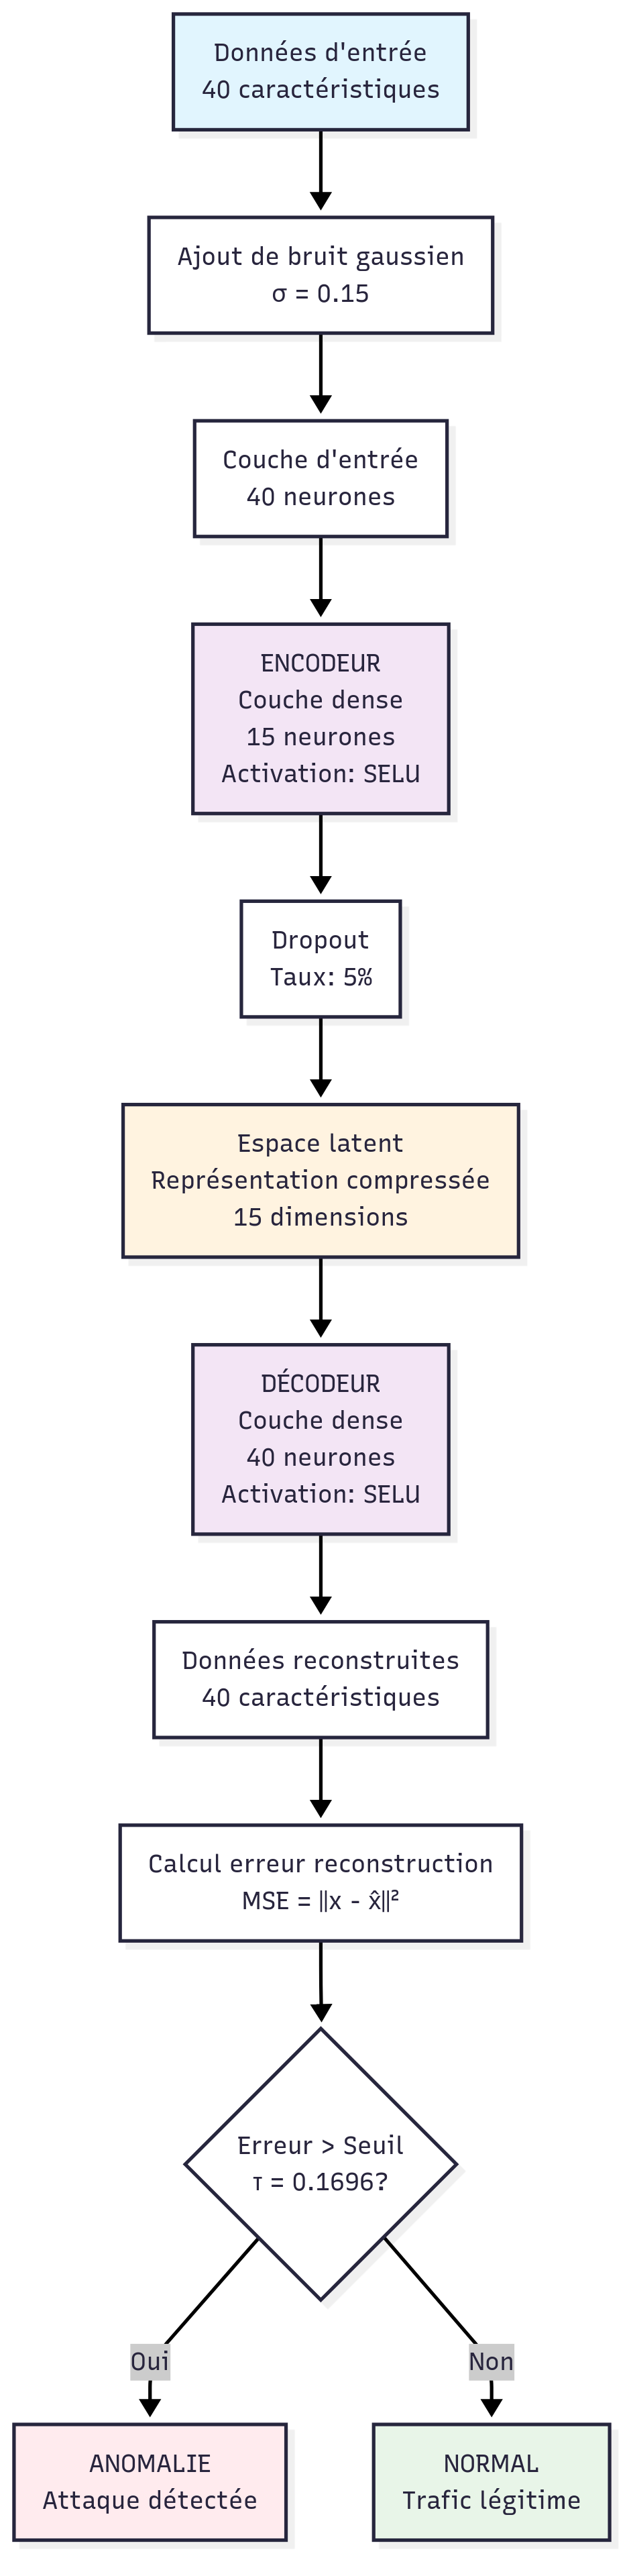
\includegraphics[width=0.3\textwidth]{Assets/autoencoder architecture.png}
    \caption{Architecture de l'autoencodeur pour la détection d'anomalies}
    \label{fig:autoencoder}
\end{figure}

\subsubsection{Architecture}
Notre autoencodeur se compose de :
\begin{itemize}
    \item \textbf{Couche d'entrée} : 41 neurones avec bruit gaussien $\mathcal{N}(0, 0.15^2)$
    \item \textbf{Couche d'encodage} : 15 neurones avec activation SELU et dropout (5\%)
    \item \textbf{Couche de décodage} : 41 neurones avec activation SELU
\end{itemize}

\subsubsection{Fonction d'activation SELU}
La fonction SELU (Scaled Exponential Linear Unit) est définie par :

\begin{equation}
    \text{SELU}(x) = \lambda \begin{cases}
        x & \text{si } x > 0 \\
        \alpha(e^x - 1) & \text{si } x \leq 0
    \end{cases}
\end{equation}

avec $\alpha = 1.6732632423543772$ et $\lambda = 1.0507009873554805$.

\subsubsection{Fonction de coût}
L'erreur quadratique moyenne (MSE) est utilisée comme fonction de coût :

\begin{equation}
    \mathcal{L}_{\text{MSE}} = \frac{1}{n}\sum_{i=1}^{n}\|\mathbf{x}_i - \hat{\mathbf{x}}_i\|^2
\end{equation}

\subsubsection{Détection d'anomalies}
L'erreur de reconstruction pour un échantillon $\mathbf{x}$ est :

\begin{equation}
    \text{erreur\_reconstruction}(\mathbf{x}) = \|\mathbf{x} - \mathbf{\hat{x}}\|^2
\end{equation}

Le seuil de détection est défini comme le 95ème percentile des erreurs de reconstruction sur les données normales :

\begin{equation}
    \tau = \text{percentile}_{95}(\{\text{erreur\_reconstruction}(\mathbf{x}_i) : y_i = \text{normal}\})
\end{equation}

\subsection{Réseau de neurones profond pour classification multi-classes}

\subsubsection{Architecture}
Le DNN comprend :
\begin{itemize}
    \item \textbf{Couche d'entrée} : 41 neurones
    \item \textbf{Première couche cachée} : 80 neurones, ReLU, dropout (30\%)
    \item \textbf{Seconde couche cachée} : 40 neurones, ReLU, dropout (20\%)
    \item \textbf{Couche de sortie} : 4 neurones, softmax
\end{itemize}

\subsubsection{Fonction de coût}
L'entropie croisée sparse est utilisée :

\begin{equation}
    \mathcal{L} = -\frac{1}{N}\sum_{i=1}^{N} \log(p_{y_i})
\end{equation}

\section{Stratégie hiérarchique}

\subsection{Étape 1 : Classification binaire}

La première étape distingue le trafic normal des activités malveillantes. Nous évaluons tous les algorithmes présentés et sélectionnons le plus performant.

\subsection{Étape 2 : Classification des types d'attaques}

Cette étape utilise uniquement les échantillons classifiés comme malveillants, permettant une spécialisation sur la discrimination entre types d'attaques.

\section{Gestion du déséquilibre : SVM-SMOTE}

\subsection{Algorithme SVM-SMOTE}

SVM-SMOTE améliore SMOTE en utilisant un SVM pour identifier les échantillons critiques :

\begin{enumerate}
    \item Entraîner un SVM sur les données déséquilibrées
    \item Identifier les vecteurs de support de la classe minoritaire
    \item Pour chaque vecteur de support $\mathbf{x}_i$ :
    \begin{enumerate}
        \item Trouver ses $k$ plus proches voisins de la même classe
        \item Générer des échantillons synthétiques par interpolation :
        \begin{equation}
            \mathbf{x}_{\text{new}} = \mathbf{x}_i + \lambda \cdot (\mathbf{x}_j - \mathbf{x}_i)
        \end{equation}
        où $\lambda \sim \mathcal{U}(0,1)$ et $\mathbf{x}_j$ est un voisin choisi aléatoirement
    \end{enumerate}
\end{enumerate}

\begin{figure}[H]
    \centering
    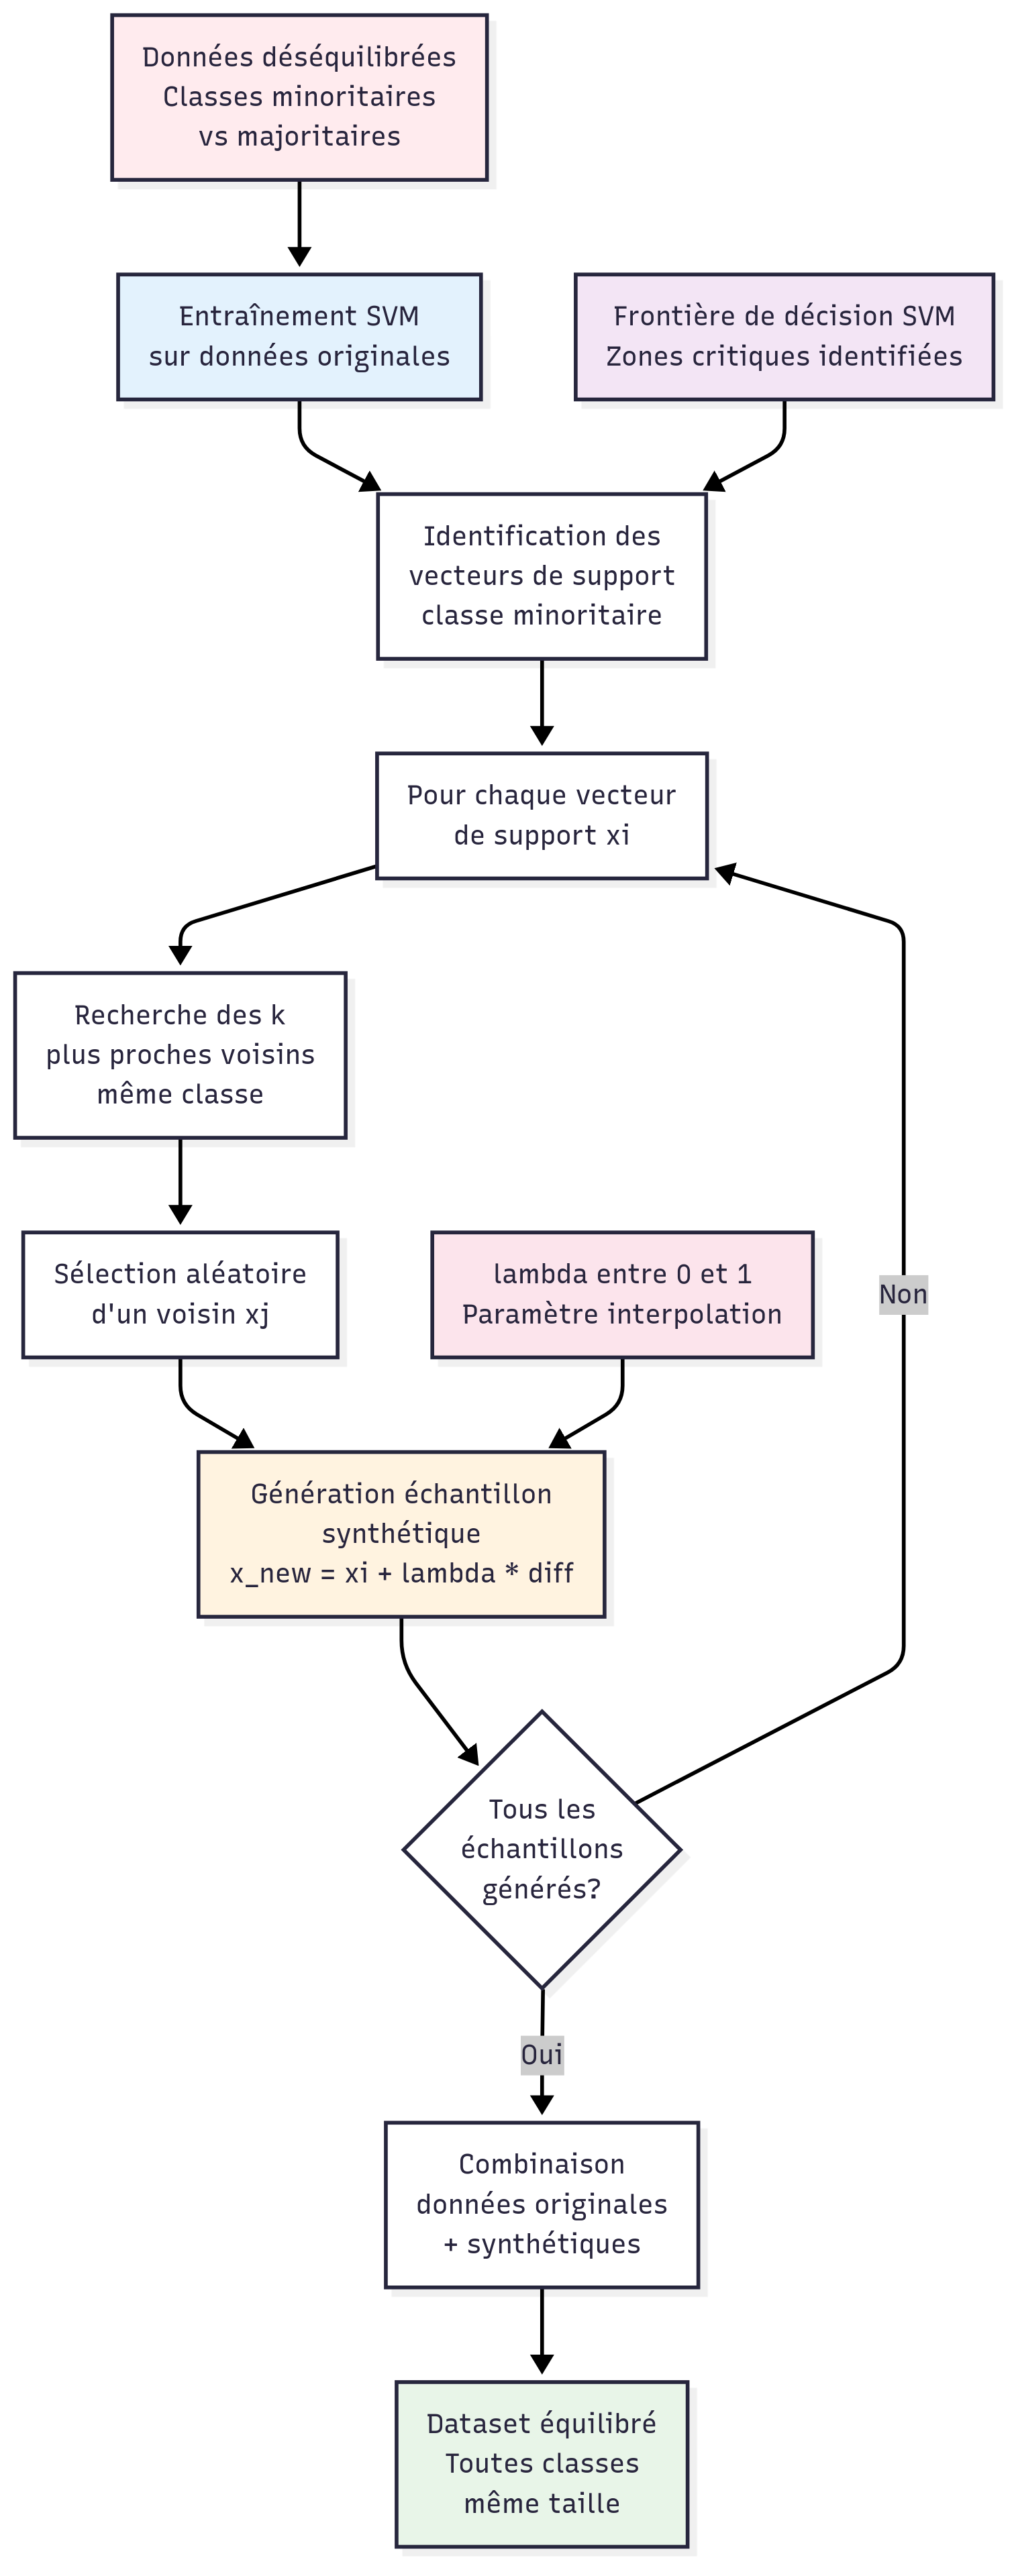
\includegraphics[width=0.4 \textwidth]{Assets/Illustration du processus SVM-SMOTE.png}
    \caption{Illustration du processus SVM-SMOTE}
    \label{fig:smote}
\end{figure}

\section{Métriques d'évaluation}

\subsection{Métriques de base}

\begin{align}
    \text{Précision} &= \frac{TP}{TP + FP} \\
    \text{Rappel} &= \frac{TP}{TP + FN} \\
    \text{F1-score} &= \frac{2 \times \text{Précision} \times \text{Rappel}}{\text{Précision} + \text{Rappel}} \\
    \text{Exactitude} &= \frac{TP + TN}{TP + TN + FP + FN}
\end{align}

\subsection{Métriques agrégées}

\begin{align}
    \text{F1-macro} &= \frac{1}{K}\sum_{k=1}^{K} \text{F1-score}_k \\
    \text{F1-micro} &= \frac{2 \times \text{Précision}_{\text{micro}} \times \text{Rappel}_{\text{micro}}}{\text{Précision}_{\text{micro}} + \text{Rappel}_{\text{micro}}}
\end{align}

Cette méthodologie complète assure une évaluation rigoureuse et reproductible de notre système de détection d'intrusions hiérarchique.

\newpage